\documentclass[lang=cn,10pt]{elegantbook}
\usepackage{graphicx}
\usepackage{float}
\usepackage{gensymb}
\usepackage{txfonts}
\setmainfont{TeX Gyre Termes}
\title{数分}



\author{ Huang}



\setcounter{tocdepth}{3}


\cover{cover.jpg}
% 本文档命令
\usepackage{array}
\newcommand{\ccr}[1]{\makecell{{\color{#1}\rule{1cm}{1cm}}}}

% 修改标题页的橙色带
% \definecolor{customcolor}{RGB}{32,178,170}
% \colorlet{coverlinecolor}{customcolor}

\begin{document}
	
	\maketitle
	\frontmatter
	
	\mainmatter
	\begin{theorem}[$Bolzano-Weierstrass $致密性定理]
		$\mathbb{R} ^n$中的集合 $E$
		是列紧集的充要条件是 $E$ 为有界闭集
	\end{theorem}
	\begin{proof}
		
		$\Rightarrow$
		
		先证明有界($ps.$其实列紧性和紧致性是等价的)、
		
		正面做不好做,我们反证法
		
		假设其发散
		
		\begin{equation*}
			\forall M>0,\exists x\in E,\text{使得}\left\| x \right\| >M
		\end{equation*}
		
		接下来的手法需要积累
		
		取$M=1$,$\exists x_{1}\in E,\text{使得}\left\| x \right\| >M$
		
		取$M=\max \left\{ 2,\left\| x_1 \right\| +1 \right\} $,$\exists x_{2}\in E,\text{使得}\left\| x_{2} \right\| >M$
		
		$\cdots$
		
		取$M=\max \left\{ k,\left\| x_{k-1} \right\| +1 \right\} $,$\exists x_{k}\in E,\text{使得}\left\| x_{k} \right\| >M$
		
		这样取,构成了一个集合$\left\{ x_n \right\} 
		$
		
		由于$\left\{ x_n \right\} 
		\subset E$是列紧集,故可选取子列使其收敛,不妨选取
		$\left\{ x_{n_{k}} \right\} 
		\subset\left\{ x_n \right\} 
		\subset E$,其中$\left\{ x_{n_{k}} \right\} $收敛
		
		但事实上,$\exists N,n_{k_{1}}> n_{k_{2}}>N$
		\begin{equation*}
			\left\| x_{n_{k_1}}-x_{n_{k_2}} \right\| >n_{k_1}-n_{k_2}
		\end{equation*}
		
		此时发散,与子列收敛矛盾
		
		再证明其为闭集
		
		只需证明$E$中所有收敛数列的极限都收敛到$E$中即可
		
		$\text{取}\left\{ x_n \right\} \subset E,\text{并且}\underset{n\rightarrow \infty}{\lim}x_n=x$
		
		对于$\left\{ x_n \right\}$,我们有
		\begin{equation*}
			\forall \varepsilon>0 ,\exists N_{1},n>N_{1}\Rightarrow \left\| x_n-x \right\| <\varepsilon
		\end{equation*}
		
		下证$x\in E$
		
		由于$E$是列紧集,则
		\begin{equation*}
			\exists \left\{ x_{n_{k}} \right\}\subset\left\{ x_n \right\},\text{使得}\underset{n\rightarrow \infty}{\lim}x_{_{n_{k}}}=x_{0}\in E
		\end{equation*}
		
		即
		
		\begin{equation*}
			\forall \varepsilon>0 ,\exists N_{2},n>N_{2}\Rightarrow \left\| x_{n_{k}}-x_{0} \right\| <\varepsilon
		\end{equation*}
		
		由于$x_{n_{k}}$为$x_{n}$子列,且$x_{n}$收敛
		,则有
		
		\begin{equation*}
			\forall \varepsilon>0 ,\exists N_{3},n>N_{3}\Rightarrow \left\| x_{n_{k}}-x_{n} \right\| <\varepsilon
		\end{equation*}
		
		取$N=\max \left\{ N_1,N_2,N_3 \right\} $
		\begin{equation*}
			\forall \varepsilon >0,n>N,\text{有}\left\| x-x_0 \right\| =\left\| x-x_n+x_n-x_{n_k}+x_{n_k}-x_0 \right\| <3\varepsilon 
		\end{equation*}
		则$x\in E$
		
		$\Leftarrow$
		
		由于$E$为有界闭集,则
		\begin{equation*}
			\forall x\in E,\exists \left\{ x_{n_k} \right\} \subset \left\{ x_n \right\} \subset E,\text{使得}\underset{n\rightarrow \infty}{\lim}x_{n_k}=x\in E
		\end{equation*}
		
		由此,$E$是列紧集
	\end{proof}
	\begin{theorem}[$Heine-Borel$ 有限覆盖定理]
		$ \mathbb{R} ^n$中的集合 $E$ 是紧致
		集的充要条件是 $E$ 为有界闭集
	\end{theorem}
	\begin{proof}
		
		$\Rightarrow$
		
		先证明有界
		
		由题,我们可以构造以下开覆盖
		\begin{equation*}
			\bigcup_{i=1}^{+\infty}{B\left( 0,i \right)}
		\end{equation*}
		
		显然有
		\begin{equation*}
			E\subset\mathbb{R} ^n \subset	\bigcup_{i=1}^{+\infty}{B\left( 0,i \right)}
		\end{equation*}
		
		由有限覆盖定理,$\exists m>0$使得
		\begin{equation*}
			E\subset	\bigcup_{i=1}^{m}{B\left( 0,i \right)}
		\end{equation*}
		
		显然有
		\begin{equation*}
			B(0,i)\subset B(0,i+1)
		\end{equation*}
		
		于是
		\begin{equation*}
			E\subset	\bigcup_{i=1}^{m}{B\left( 0,i \right)}=B(0,m)
		\end{equation*}
		由于$ B(0,m)$有界,于是$E$有界
		
		再证明其为闭集合(这题的手法也很不错,大家积累积累)
		
		要证为闭集合,只需证明其补集$E^{c}$为开集即可,
		即
		\begin{equation*}
			\forall y\in E^c,\exists r_1>0,\text{使得}B\left( y,r_1 \right) \subset E^c
		\end{equation*}
		
		由$Hausdorff$定理
		\begin{equation*}
			\forall x\in E,\exists \delta _x,\eta _x>0,\text{使得}B\left( x,\delta _x \right) \cap B\left( y,\eta _x \right) =\oslash 
		\end{equation*}
		
		显然有
		\begin{equation*}
			\bigcup_{x\in E}{B\left( x,\delta _x \right)}\supset \bigcup_{x\in E}{x}=E
		\end{equation*}
		
		由紧致性,我们有
		\begin{equation*}
			\bigcup_{i=1}^m{B\left( x_i,\delta _i \right)}\supset \bigcup_{x\in E}{x}=E
		\end{equation*}
		
		于是乎,取$r=\min \left\{ \eta _{x_1},\eta _{x_2},\cdots ,\eta _{x_m} \right\} $,我们有
		\begin{equation*}
			B\left( y,r \right) \cap \bigcup_{i=1}^m{B\left( x_i,\delta _i \right)}=\oslash \supset B\left( y,r \right) \cap \bigcup_{x\in E}{x}=E
		\end{equation*}
		
		因此,我们有
		\begin{equation*}
			B\left( y,r \right) \cap E=\oslash
		\end{equation*}
		
		故
		\begin{equation*}
			B\left( y,r \right) \subset E^{c}
		\end{equation*}
		
		$\Leftarrow$(可以参考习题1.9,这里给出课上的做法)
		
		我们反证,由于其为有界闭集,则存在一个矩形将该区间包住,
		\begin{figure}[H]
			\centering
			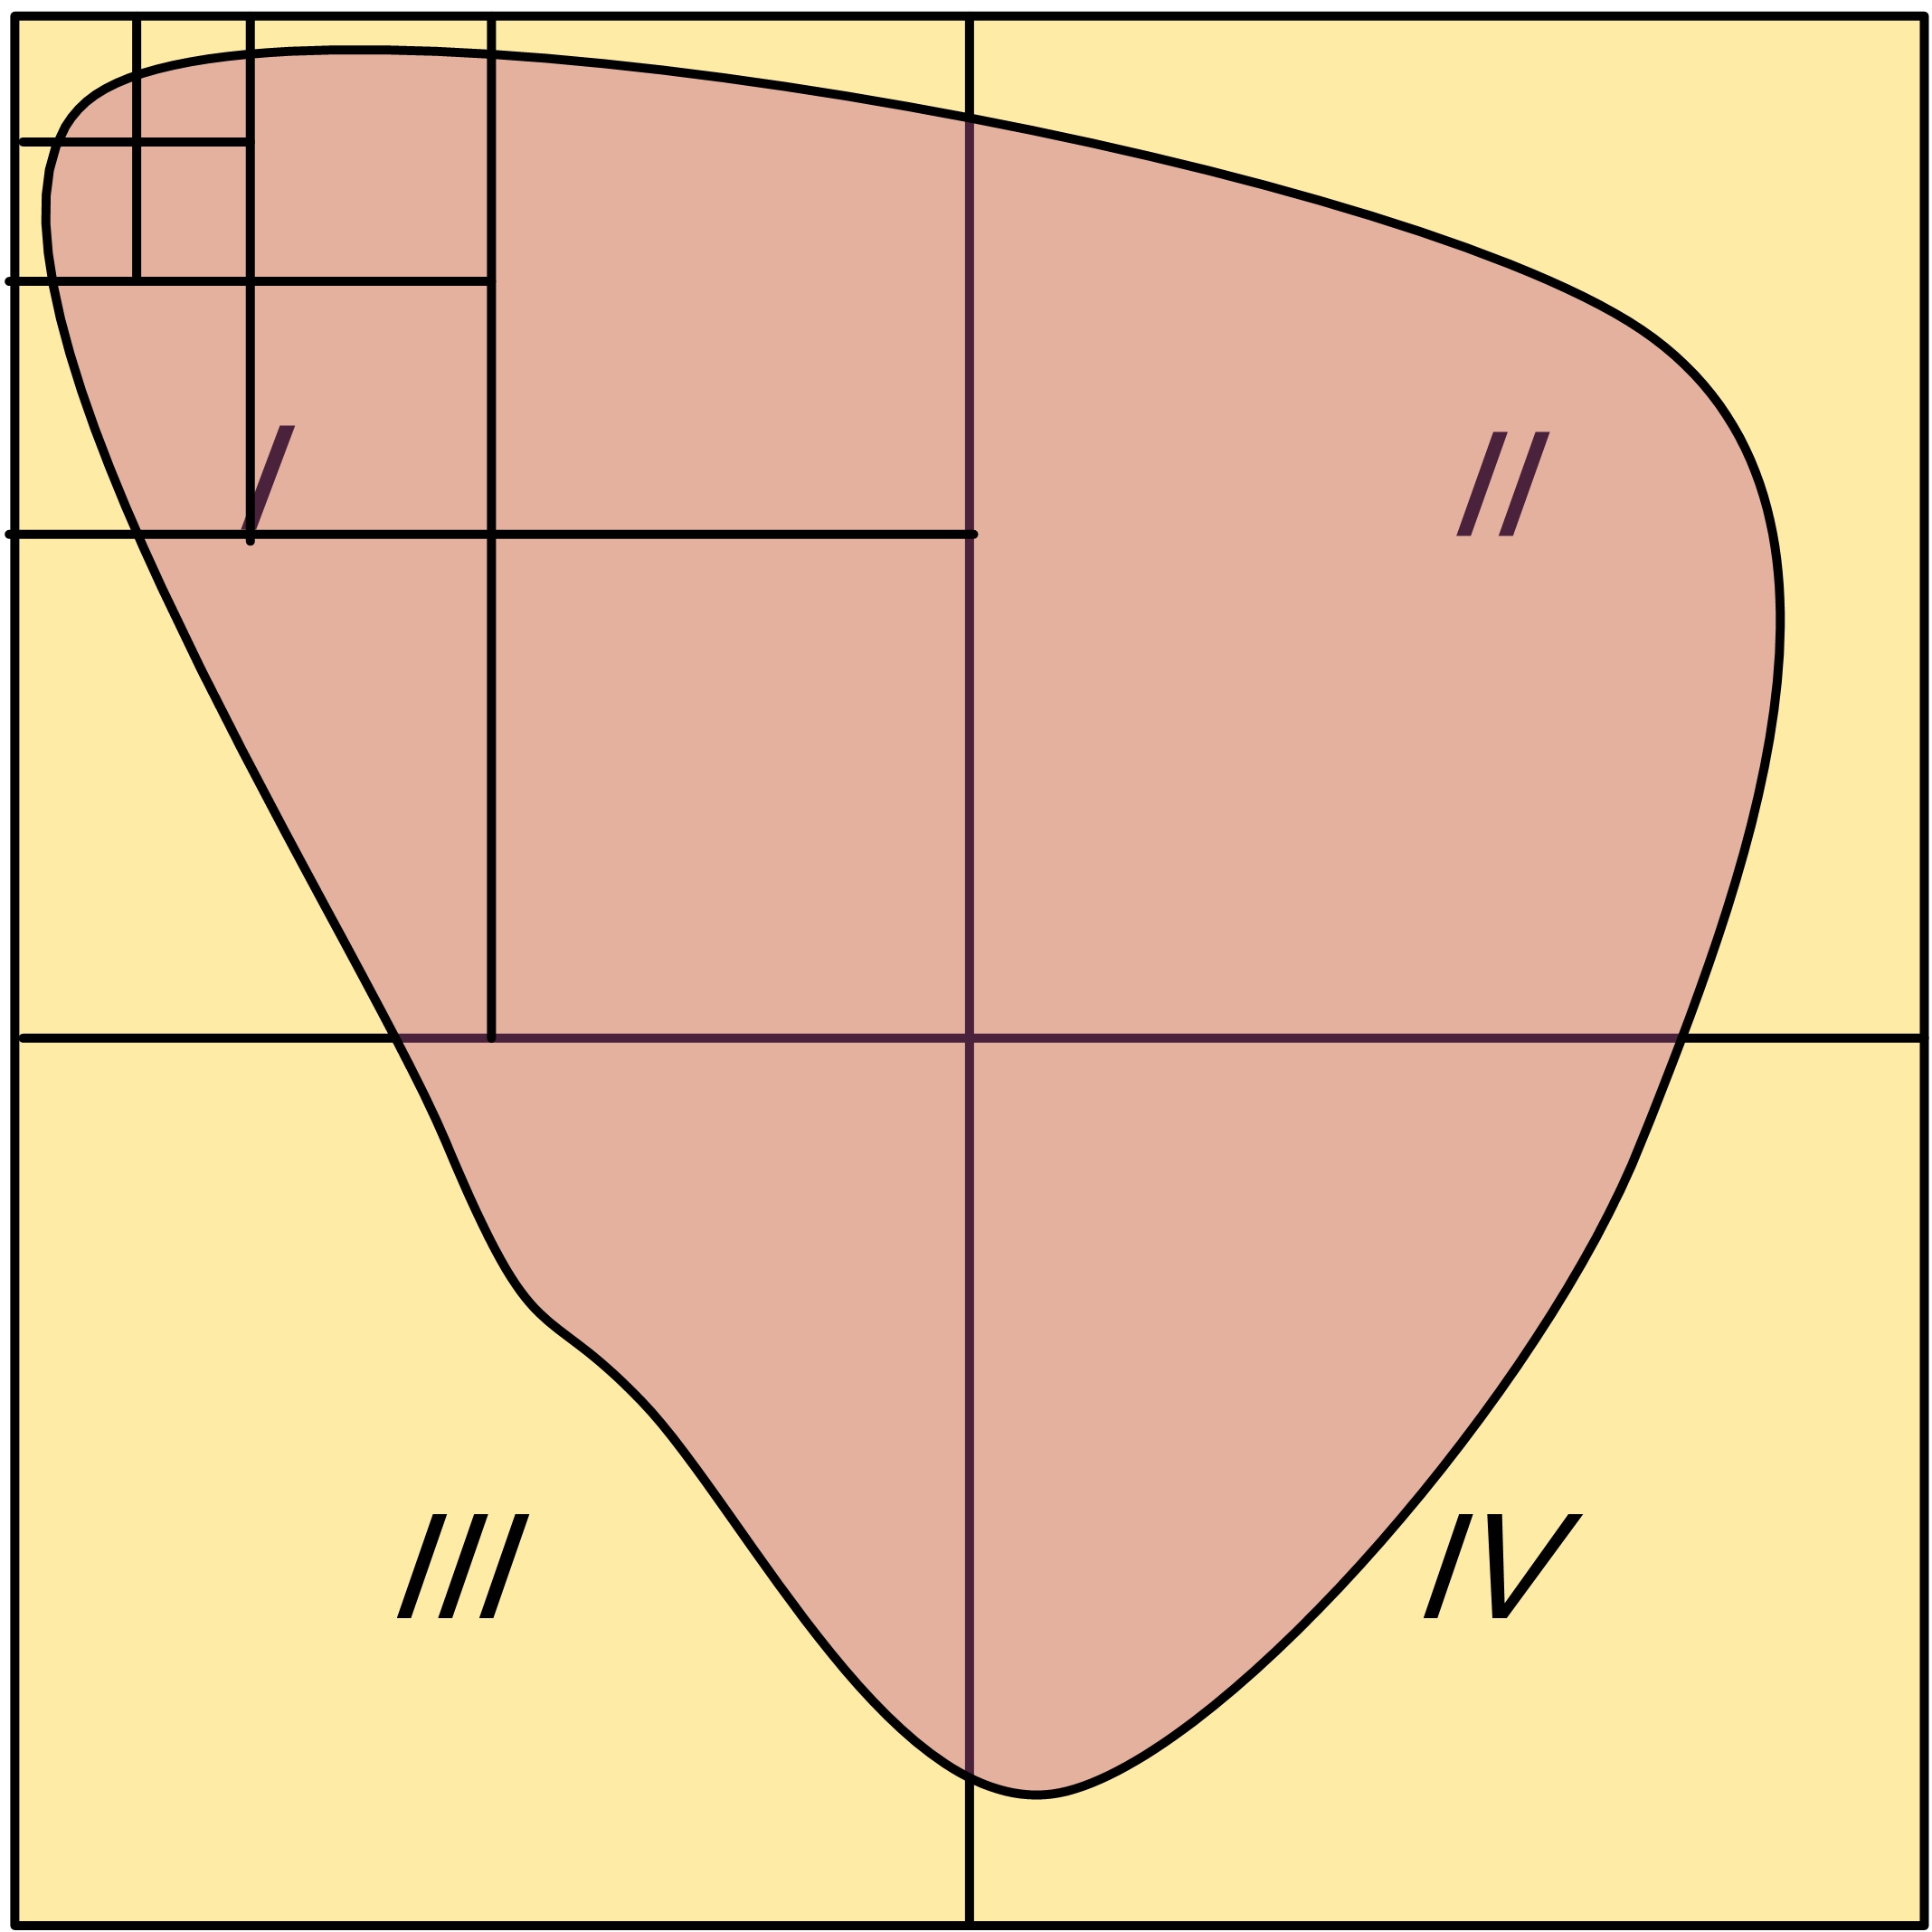
\includegraphics[width=0.2\linewidth]{Untitled}
			\caption{}
			\label{fig:untitled}
		\end{figure}
		
		如图(1.1),我们将其该矩形四等分,则存在一些区域无法被有限个开覆盖覆盖,不失一般性,不妨假设是在Ⅰ区在一区中,我们将其四等分,同样能找到不能被有限个开覆盖覆盖的区域,类似的,我们多次将其四等分,构成了一系列的非空的区间套,这些区间不能被有限个开覆盖覆盖,由区间套定理,我们可以找到一个唯一的$x\in E$,并且其不能被有限个开区间覆盖,但显然$B(x,\delta)$可覆盖住$x$,矛盾。于是原命题得证
	\end{proof}
	\begin{theorem}
		道路连通集一定是连通集
	\end{theorem}
	\begin{proof}
		
		不妨设$E$道路连通,下证其为连通集
		
		令\begin{equation*}
			E=A\cup B;A,B\ne \oslash ;A\cap B=\oslash 
		\end{equation*}
		
		只需证明
		\begin{equation*}
			A\cap B'\ne\oslash\text{或}B\cap A'\ne\oslash
		\end{equation*}
		
		即可
		
		取$p\in A,q\in B$,由于$E$道路连通,则存在一个向量函数$\Phi \left( t \right) ,t\in \left[ 0,1 \right] $,使得
		\begin{equation*}
			\Phi \left( 0 \right)=p,\Phi \left( 1 \right)=q
		\end{equation*}
		令$\begin{cases}
			S=\left\{ t\in \left[ 0,1 \right] |\Phi \left( t \right) \in A \right\}\\
			T=\left\{ t\in \left[ 0,1 \right] |\Phi \left( t \right) \in B \right\}\\
		\end{cases}$
		
		显然有
		\begin{equation*}
			S\cup T=\left[ 0,1 \right] ,S\ne \oslash ,T\ne \oslash ,S\cap T=\oslash 
		\end{equation*}
		(这里我们采用了一种部分代替整体的手法,可以积累一下)
		
		由于[0,1]为连通的,则有
		\begin{equation*}
			S\cap T'\ne\oslash\text{或}T\cap S'\ne\oslash
		\end{equation*}
		
		不妨设$S\cap T'\ne \oslash \text{,取}x\in S\cap T',\text{则有}\left\{ x_n \right\} \subset T,\text{使得}\lim_{n\rightarrow \infty} x_n=x\left( x_n\ne x \right)$ 
		
		于是有
		\begin{equation*}
			\Phi \left( x \right)\in A,\Phi \left( x_{n} \right)\in B
		\end{equation*}
		
		由于$\Phi \left( t \right)$连续,则
		\begin{equation*}
			|\Phi\left( x_{n} \right)-\Phi \left( x \right)|<\varepsilon
		\end{equation*}
		于是$\Phi \left( x \right)\in B'$,结论得证
	\end{proof}
	\begin{theorem}
		$\text{设}D\subset \mathbb{R} ^n,f:D\rightarrow \mathbb{R}$,且 $f$ 在 $D$ 上连续,如果 $D$
		是紧集,则 $f$ 的值域 $f(D) $也是紧集
	\end{theorem}
	\begin{proof}
		要证明这个定理,我们需要用到两个个引理(一个?)
		\begin{lemma}
			$\text{函数}f\text{:}\mathbb{R} ^n\rightarrow \mathbb{R} ,\text{连续的充要条件是对于}\mathbb{R} \text{中的任意开集}U\text{,}f^{-1}(U)\text{为}\mathbb{R} ^n\text{中的开集。}$
			
		\end{lemma}
		\begin{lemma}
			设 $X$ 为拓扑空间,$Y $为 $X$ 的紧致子集的充要条件是
			对每个由 $X $中的开集构成的 $Y $的覆盖均有有限子覆盖(我证明好像没用上这个,就不证明了OVO)
		\end{lemma}
		
		现我们开始证明
		
		$\text{我们任取}f\left( D \right) \text{的开覆盖}\left\{ U_{\alpha} \right\} \left( \alpha \in I \right) \text{,由引理2.1,我们有}f^{-1}\left( U_{\alpha} \right) \left( \alpha \in I \right) \text{均为开集}
		$
		
		因为
		\begin{equation*}
			\bigcup_{\alpha \in I}{U_{\alpha}}\supset f\left( D \right) 
		\end{equation*}
		
		我们将左右两边同时作用$f^{-1}$算子,有
		\begin{equation*}
			f^{-1}(\bigcup_{\alpha \in I}{U_{\alpha}})\supset f^{-1}(f\left( D \right)) =D
		\end{equation*}
		
		猜想:若
		\begin{equation*}
			\bigcup_{\alpha \in I}{f^{-1}\left( U_{\alpha} \right)}\supset f^{-1}(\bigcup_{\alpha \in I}{U_{\alpha}})\supset f^{-1}(f\left( D \right) )=D
		\end{equation*}
		成立
		
		由于$D$为紧集,则$\bigcup_{\alpha \in I}{f^{-1}\left( U_{\alpha} \right)}
		$存在有限子覆盖,不妨记为
		\begin{equation*}
			\bigcup_{i=1}^m{f^{-1}\left( U_i \right)}
		\end{equation*}
		
		此时若
		\begin{equation*}
			\bigcup_{i=1}^m{f(f^{-1}\left( U_i \right))}=\bigcup_{i=1}^m{U_i}
		\end{equation*}
		构成$f(D)$的有限覆盖,则命题得证
		
		不妨设其不能称为$f(D)$的有限子覆盖,则
		\begin{equation*}
			\exists x \in f(D),x\notin \bigcup_{i=1}^m{f(f^{-1}\left( U_i \right))}=\bigcup_{i=1}^m{U_i}
		\end{equation*}
		
		同时作用$f^{-1}$算子,我们有
		\begin{equation*}
			\exists f^{-1}(x)\in f^{-1}(f(D))=D,f^{-1}(x)\notin f^{-1}(\bigcup_{i=1}^m{f(f^{-1}\left( U_i \right))})=f^{-1}(\bigcup_{i=1}^m{U_i})
		\end{equation*}
		
		但
		\begin{equation*}
			\forall y\in f(D),\exists i ,\text{使得}f^{-1}(y)\in f^{-1}(U_{i})
		\end{equation*}
		故矛盾,命题得证
		
		下证猜想
		\begin{equation*}
			\bigcup_{\alpha \in I}{f^{-1}\left( U_{\alpha} \right)}\supset f^{-1}(\bigcup_{\alpha \in I}{U_{\alpha}})
		\end{equation*}
		\begin{equation*}
			\forall x\in f^{-1}(\bigcup_{\alpha \in I}{U_{\alpha}}),\text{存在}\alpha ,\text{我们有}f\left( x \right) \in U_{\alpha},\text{故}x\in f^{-1}\left( U_{\alpha} \right) \subset \bigcup_{\alpha \in I}{f^{-1}\left( U_{\alpha} \right)}
		\end{equation*}
		
		得证
		
		下证引理(2.1)
		\begin{proof}
			
			$\Rightarrow$
			
			若$f^{-1}(U)=\oslash $,显然为开集
			
			若$f^{-1}(U)\ne\oslash $,我们取$\forall x \in f^{-1}(U)$,则有$f(x)\in U$
			
			由于$U$为开集,则有
			\begin{equation*}
				\exists \varepsilon ,B(f(x),\varepsilon)\subset U
			\end{equation*}
			
			又因为$f$连续,则有
			\begin{equation*}
				f\left( B\left( x,\delta \right) \right) \subset B\left( f\left( x \right) ,\varepsilon \right) \subset U
			\end{equation*}
			
			同时作用$f^{-1}$,则有
			
			\begin{equation*}
				B\left( x,\delta \right) \subset f^{-1}\left( B\left( f\left( x \right) ,\varepsilon \right) \right) \subset f^{-1}\left( U \right) 
			\end{equation*}
			
			$\Leftarrow$
			
			任意$x\in f^{-1}(U)$取$B(f(x),\varepsilon) \subset U$,则有
			\begin{equation*}
				f^{-1}(B(f(x),\varepsilon)) \text{为开集}
			\end{equation*}
			
			又有$x\in f^{-1}(B(f(x),\varepsilon))$,
			则有
			\begin{equation*}
				\exists \delta>0,B(x,\delta)\subset f^{-1}(B(f(x),\varepsilon))
			\end{equation*}
			
			于是有
			\begin{equation*}
				f(B(x,\delta))\subset B(f(x),\varepsilon)
			\end{equation*}
			得证
		\end{proof}
	\end{proof}
	\begin{theorem}
		$\text{设}D\subset \mathbb{R} ^n$是连通集,$f:D\rightarrow \mathbb{R}$,且 $f$ 在 $D$ 上连续,则
		$f(D)$ 是 $\mathbb{R}$ 上的连通集
	\end{theorem}
	\begin{proof}
		
		直接硬来,取$f(D)=A\cup B,A\cap B=\oslash$
		\begin{equation*}
			\text{记}G=D\cap f^{-1}\left( A \right) ,F=D\cap f^{-1}\left( B \right) 
		\end{equation*}
		
		我们有
		\begin{equation*}
			D=G\cup F
		\end{equation*}
		
		$\text{由}A\subset \bar{A},\text{我们有}G=D\cap f^{-1}\left( A \right) \subset f^{-1}(\bar{A}),\text{由于}f\text{连续},\bar{A}\text{为闭集},\text{我们有}f^{-1}\left( \bar{A} \right) \text{为闭集}$对前一式子取闭包,我们有
		\begin{equation*}
			\bar{G}\subset \overline{f^{-1}(\bar{A})}=f^{-1}\left( \bar{A} \right) 
		\end{equation*}
		
		因此,我们有
		\begin{equation*}
			f\left( \bar{G} \right) \subset f\left( f^{-1}\left( \bar{A} \right) \right) =\bar{A}
		\end{equation*}
		
		现在我们只需要证明$A'\cap B\ne \oslash$即可,不妨证明逆否命题,加上$A\cap B=\oslash$的条件,我们有
		\begin{equation*}
			\bar{A}\cap B=\oslash,\text{即}f\left( \bar{G} \right) \cap B=\oslash 
		\end{equation*}
		
		显然有
		\begin{equation*}
			B\supset f\left( F \right) 
		\end{equation*}
		
		于是,我们有
		\begin{equation*}
			\forall y\in B\subset f\left( D \right) ,f^{-1}\left( y \right) \in F=D\cap f^{-1}\left( B \right) \Rrightarrow y\in f\left( F \right) 
		\end{equation*}
		
		因此,我们有
		\begin{equation*}
			B=f\left( F \right) 
		\end{equation*}
		
		此时
		\begin{equation*}
			f\left( \bar{G} \right) \cap B=f\left( \bar{G} \right) \cap f\left( F \right) =\oslash \Rrightarrow \bar{G}\cap F=\oslash 
		\end{equation*}
		
		逆否命题得证
	\end{proof}
\end{document}